% Options for packages loaded elsewhere
\PassOptionsToPackage{unicode}{hyperref}
\PassOptionsToPackage{hyphens}{url}
%
\documentclass[
  9pt,
  ignorenonframetext,
]{beamer}
\usepackage{pgfpages}
\setbeamertemplate{caption}[numbered]
\setbeamertemplate{caption label separator}{: }
\setbeamercolor{caption name}{fg=normal text.fg}
\beamertemplatenavigationsymbolsempty
% Prevent slide breaks in the middle of a paragraph
\widowpenalties 1 10000
\raggedbottom
\setbeamertemplate{part page}{
  \centering
  \begin{beamercolorbox}[sep=16pt,center]{part title}
    \usebeamerfont{part title}\insertpart\par
  \end{beamercolorbox}
}
\setbeamertemplate{section page}{
  \centering
  \begin{beamercolorbox}[sep=12pt,center]{part title}
    \usebeamerfont{section title}\insertsection\par
  \end{beamercolorbox}
}
\setbeamertemplate{subsection page}{
  \centering
  \begin{beamercolorbox}[sep=8pt,center]{part title}
    \usebeamerfont{subsection title}\insertsubsection\par
  \end{beamercolorbox}
}
\AtBeginPart{
  \frame{\partpage}
}
\AtBeginSection{
  \ifbibliography
  \else
    \frame{\sectionpage}
  \fi
}
\AtBeginSubsection{
  \frame{\subsectionpage}
}
\usepackage{lmodern}
\usepackage{amsmath}
\usepackage{ifxetex,ifluatex}
\ifnum 0\ifxetex 1\fi\ifluatex 1\fi=0 % if pdftex
  \usepackage[T1]{fontenc}
  \usepackage[utf8]{inputenc}
  \usepackage{textcomp} % provide euro and other symbols
  \usepackage{amssymb}
\else % if luatex or xetex
  \usepackage{unicode-math}
  \defaultfontfeatures{Scale=MatchLowercase}
  \defaultfontfeatures[\rmfamily]{Ligatures=TeX,Scale=1}
\fi
\usetheme[]{Goettingen}
\usecolortheme{rose}
% Use upquote if available, for straight quotes in verbatim environments
\IfFileExists{upquote.sty}{\usepackage{upquote}}{}
\IfFileExists{microtype.sty}{% use microtype if available
  \usepackage[]{microtype}
  \UseMicrotypeSet[protrusion]{basicmath} % disable protrusion for tt fonts
}{}
\makeatletter
\@ifundefined{KOMAClassName}{% if non-KOMA class
  \IfFileExists{parskip.sty}{%
    \usepackage{parskip}
  }{% else
    \setlength{\parindent}{0pt}
    \setlength{\parskip}{6pt plus 2pt minus 1pt}}
}{% if KOMA class
  \KOMAoptions{parskip=half}}
\makeatother
\usepackage{xcolor}
\IfFileExists{xurl.sty}{\usepackage{xurl}}{} % add URL line breaks if available
\IfFileExists{bookmark.sty}{\usepackage{bookmark}}{\usepackage{hyperref}}
\hypersetup{
  pdftitle={BIOS6643 Longitudinal},
  pdfauthor={EJC},
  hidelinks,
  pdfcreator={LaTeX via pandoc}}
\urlstyle{same} % disable monospaced font for URLs
\newif\ifbibliography
\setlength{\emergencystretch}{3em} % prevent overfull lines
\providecommand{\tightlist}{%
  \setlength{\itemsep}{0pt}\setlength{\parskip}{0pt}}
\setcounter{secnumdepth}{-\maxdimen} % remove section numbering
\AtBeginSubsection{}
\AtBeginSection{}
\ifluatex
  \usepackage{selnolig}  % disable illegal ligatures
\fi

\title{BIOS6643 Longitudinal}
\subtitle{L22 Extra Topics}
\author{EJC}
\date{}
\institute{Department of Biostatistics \& Informatics}

\begin{document}
\frame{\titlepage}

\begin{frame}[allowframebreaks]
  \tableofcontents[hideallsubsections]
\end{frame}
\hypertarget{extra-topics}{%
\section{Extra topics}\label{extra-topics}}

\begin{frame}{Topics}
\protect\hypertarget{topics}{}
\begin{itemize}
\item
  Causal inference and marginal structural models
\item
  Measurement error methods
\item
  Basics of spatial methods: kriging
\end{itemize}

\textbf{The full slide sets are also posted on Canvas (see extra sets)}
\end{frame}

\begin{frame}{}
\protect\hypertarget{section}{}
We will walk through the following questions:

\begin{itemize}
\item
  What is it?
\item
  Why is it important?
\item
  When is it important to use?
\item
  How are methods used/applied?
\item
  How does it apply to longitudinal data?
\end{itemize}
\end{frame}

\hypertarget{causal-inference-and-marginal-structural-models}{%
\section{Causal inference and marginal structural
models}\label{causal-inference-and-marginal-structural-models}}

\begin{frame}{Causal inference and marginal structural models}
\protect\hypertarget{causal-inference-and-marginal-structural-models-1}{}
\begin{block}{What is it?}
\protect\hypertarget{what-is-it}{}
Causal inference contains the set of methods that attempt to show how
one variable causes change in another one.
\end{block}

\begin{block}{Why is it important?}
\protect\hypertarget{why-is-it-important}{}
As we have learned, most statistical methods address association rather
than causation. Causation requires ruling out other variables that can
explain the association. To some degree this can be accomplished by
including covariates in regression models. However, in certain cases,
this approach does not work either.
\end{block}

\begin{block}{When is it important to use?}
\protect\hypertarget{when-is-it-important-to-use}{}
When an outcome (Y) predicts a subsequent value of an explanatory
variable (X) that can't be predicted by previous X values.

When there is a time-varying confounder (Z) that affects both X (e.g.,
treatment or exposure variable) and the outcome, and X (history) affects
subsequent values of Z.
\end{block}
\end{frame}

\begin{frame}{}
\protect\hypertarget{section-1}{}
As an example, consider asthmatic children; let

X = cigarette smoke exposure\\
Z = asthma symptoms\\
Y = inhaler use.

It is feasible that asthma symptoms not only increases the likelihood of
inhaler use, but also affects subsequent exposures (e.g., if a child
with more symptoms is less likely to be in smoke filled environment,
either based on child's or parent's behavior).

It is also feasible if not likely that the cigarette smoke exposure
`history' (i.e., within the observational study period) affects
subsequent asthma symptoms.
\end{frame}

\begin{frame}{}
\protect\hypertarget{section-2}{}
In this case, standard regression methods are not the best. If we apply
a regression model for inhaler use (Y) as a function of cigarette smoke
exposure (X) plus a symptoms covariate (Z), we can estimate the
difference of conditional effects such as

\(E(Y|X=1,\ symptoms=z)-E(Y|X=0,\ symptoms=z)\)

However the causal effect of interest is\(E(Y_1-Y_0)=E(Y_1)-E(Y_0)\)
where \(E(Y_1)\) represents the expected inhaler use for a subject
randomly assigned to receive the exposure, and \(E(Y_0)\) is the same,
but if they had not received exposure. These are marginal effects and
the primary difference between these and the conditional effects above
is due to the fact that subjects are not randomized, but rather `choose'
their treatment based on factor such as the symptoms they have.
\end{frame}

\begin{frame}{}
\protect\hypertarget{section-3}{}
\begin{block}{How are methods used/applied?}
\protect\hypertarget{how-are-methods-usedapplied}{}
Inverse probability of treatment weights are used to reconstruct data as
if subjects were randomized to treatment, and eliminates confounding
effects of symptoms.
\end{block}

\begin{block}{How does it apply to longitudinal data?}
\protect\hypertarget{how-does-it-apply-to-longitudinal-data}{}
Time-varying weights can be calculated that are compounded over time.
You can fit a usual longitudinal model (e.g., a linear mixed model for a
continuous outcome or generalized linear mixed model for a binary or
count outcome), adding a weight statement to include the constructed
IPTW's.
\end{block}
\end{frame}

\begin{frame}{}
\protect\hypertarget{section-4}{}
What you end up with is an estimate of causal relationship between X
(e.g., smoke exposure) and Y (e.g., inhaler use). In our application
(considering med use as binary rather than a count), we found that
recent smoke exposure increases odds of medication use 3 times
(Estimate=3.02, 95\% CI: 1.63 to 5.58; p=0.0004). Using the naïve
regression approach, using the same health outcome model but excluding
the weight statement and including relevant symptoms predictors yielded
an OR of 2.52 (95\% CI: 1.62 to 3.92).

Notes and summary: See the \textbf{Causal inference slides} for more
detail. If you have any questions about this, just contact me. In real
life, there might be other confounders to consider, and some might not
be measured. This is what makes this analysis particularly messy and
complicated.
\end{frame}

\hypertarget{measurement-error-models}{%
\section{Measurement error models}\label{measurement-error-models}}

\begin{frame}{Measurement error models}
\protect\hypertarget{measurement-error-models-1}{}
\begin{block}{What is it?}
\protect\hypertarget{what-is-it-1}{}
The set of methods that tell us how to account for measurement error in
regression-type models. This type of measurement error can be considered
as obtaining an observed value that does not represent the `true' value.
\end{block}

\begin{block}{Example 1:}
\protect\hypertarget{example-1}{}
X = true caloric intake; however data might be obtained via a
questionnaire and it does not represent the actual value.
(Underestimated?)
\end{block}

\begin{block}{Example 2:}
\protect\hypertarget{example-2}{}
a person has a true exposure to particulate matter on a given day (say,
averaged over 24 hours), but the value that we obtain is an estimate of
it, measured with error.
\end{block}
\end{frame}

\begin{frame}{}
\protect\hypertarget{section-5}{}
\begin{block}{Why is it important?}
\protect\hypertarget{why-is-it-important-1}{}
Using predictors with measurement error can attenuate the slope.
Measurement error methods can provide a way to correct for this
attenuation (regression calibration).

Using measured with error variables, plus instrumental variables, we can
estimate associations between a health outcome and the true (unobserved)
predictors of interest (regression calibration with instrumental
variables).
\end{block}

\begin{block}{When is it important to use?}
\protect\hypertarget{when-is-it-important-to-use-1}{}
When predictors are measured with error and you have the key variables
(including instruments) of interest.
\end{block}
\end{frame}

\begin{frame}{}
\protect\hypertarget{section-6}{}
\begin{block}{How are methods used/applied?}
\protect\hypertarget{how-are-methods-usedapplied-1}{}
Example 1 (RC): attenuation correction can be applied when you have the
residual variance in the model, plus the variance of the error on the
mismeasured predictor.

Example 2 (RCIV): regress the mismeasured predictor on an instrumental
variable in order to obtain predicted values of the unobserved variable.
Then substitute these predicted values in for `X' in the regression
model for the health outcome of interest. (There is also an alternative
but equivalent approach.)
\end{block}

\begin{block}{How does it apply to longitudinal data?}
\protect\hypertarget{how-does-it-apply-to-longitudinal-data-1}{}
Methods are applied in a similar manner.
\end{block}
\end{frame}

\begin{frame}{Background}
\protect\hypertarget{background}{}
Measurement error in variables is common in scientific studies and
experiments, although often disregarded.

The problem with measurement error is that associated estimators of
interest may be biased depending on which variables have measurement
error, and the degree of bias depends on the degree of measurement
error.

When measurement error exists, methods such as regression calibration
can be used to adjust estimators so that they are unbiased or at least
consistent for the parameter of interest.
\end{frame}

\begin{frame}{Measurement error and regression modeling}
\protect\hypertarget{measurement-error-and-regression-modeling}{}
To introduce measurement error and its impacts on regression modeling,
consider daily caloric intake, where measures W are obtained via calorie
counts from a survey that are unbiased for a true caloric intake X.

We assume that subject reports are not biased low or high, i.e.,
\(W=X+U\), where U is random error with mean 0. (In real life there
might be a tendency to underreport!)

Let's say Y is subject's body mass index (BMI), and that the
relationship between Y and X can be expressed by the model
\(Y=\beta_0+\beta_1 X+ \epsilon\). If we regress Y on \(W=X+U\) instead
of X, what can we expect the slope of W to be, relative to \(\beta_1\)?
\end{frame}

\begin{frame}{}
\protect\hypertarget{section-7}{}
In another setting, let's say that the caloric intake is actually
modeled as the outcome, and we use a predictor such as a mood level.
Here say we use V=Y+U instead of Y for caloric intake.

The following graphs simulate what we might see for regression fits for
these two settings.

\begin{center}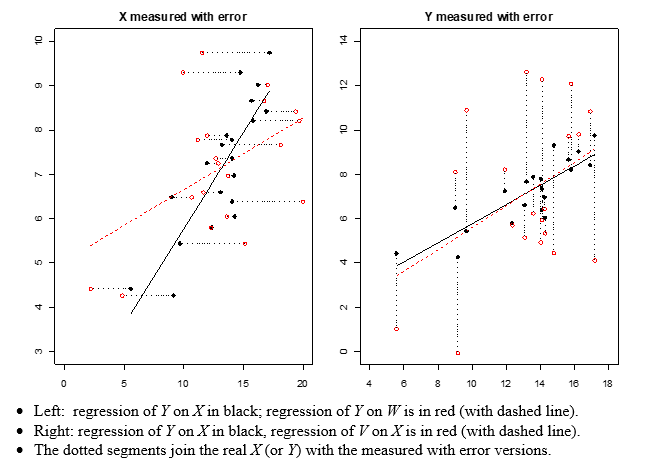
\includegraphics[width=0.7\linewidth]{figs_L22/f1} \end{center}
\end{frame}

\begin{frame}{Regression calibration with instrumental variables,
application}
\protect\hypertarget{regression-calibration-with-instrumental-variables-application}{}
We are interested in the relationship between exposure to fine
particulate matter from cigarette smoke (X1) and from ambient sources
(X2) on health outcomes of inhaler use and LTE4 (a biomarker of asthma
inflammation). For each health outcome, we build a model with
\(X1,\ X2,\ X1 \times X2\), plus covariates.

What observe `measured with error' versions of X1 and X2 (W1 and W2). We
also have instrumental variables of cotinine (M1, a biomarker of
cigarette smoke exposure) and fixed outdoor pollution (M2).

Steps: regression W1 on M1 and W2 on M2 to obtain estimated values of
\(E(X1|M1)\) and \(E(X2|M2)\). Substitute these in for X1 and X2 in the
health outcome models.
\end{frame}

\begin{frame}{}
\protect\hypertarget{section-8}{}
Findings:

\begin{itemize}
\item
  The steepest dose-reponse relationship between a pollutant and Y
  occurs when the 2nd pollutant is lower due to a significant negative
  interaction between pollutants.
\item
  We found also SHS to be more toxic than ambient pollution, comparing
  at equivalent amounts of co-exposures.
\end{itemize}
\end{frame}

\begin{frame}{Using predicted values as predictors}
\protect\hypertarget{using-predicted-values-as-predictors}{}
With the aforementioned RCIV, predicted values from one model are used
in place of unobserved values for a predictor variable in the second
model.

It needs to be kept in mind that predicted values are estimated rather
than observed, and so the variability in estimation in the first model
should be taken into account to get accurate standard errors. If
predicted values are simply placed in the 2nd model, then the standard
errors associated with slope estimates will not automatically account
for this; they tend to be underestimated.

For RCIV, we have an alternative algorithm that will make it easier to
correct the standard errors, which could be used more generally when
predicted values are used as regressors.
\end{frame}

\hypertarget{spatial-statistics-and-kriging}{%
\section{Spatial statistics and
kriging}\label{spatial-statistics-and-kriging}}

\begin{frame}{Spatial statistics and kriging}
\protect\hypertarget{spatial-statistics-and-kriging-1}{}
\begin{block}{What is it?}
\protect\hypertarget{what-is-it-2}{}
Estimation of values in a spatial (2 or 3-dimensional context). It uses
information about estimated model and correlation between points to
interpolate/extrapolate BLUP estimates for other points (e.g., for
points on a grid).
\end{block}

\begin{block}{Why is it important?}
\protect\hypertarget{why-is-it-important-2}{}
Spatial data has exploded with modern technology. These methods allow us
to interpolate estimates to obtain a more complete view of a process
using data collected at certain points. Applications: real estate, epi
applications
\end{block}

\begin{block}{When is it important to use?}
\protect\hypertarget{when-is-it-important-to-use-2}{}
When you have data collected over space, time or both. Methods that deal
with both spatial and temporal correlation are spatio-temporal methods.
\end{block}
\end{frame}

\begin{frame}{}
\protect\hypertarget{section-9}{}
\begin{block}{How are methods used/applied?}
\protect\hypertarget{how-are-methods-usedapplied-2}{}
There are different spatial methods, and many new spatio-temporal
methods. What I present here is called `kriging', which has its origins
in estimators obtained from simpler linear mixed models.
\end{block}

\begin{block}{How does it apply to longitudinal data?}
\protect\hypertarget{how-does-it-apply-to-longitudinal-data-2}{}
It applies when you consider spatio-temporal data and methods. However,
if you are talking about correlated data models, spatial data fall into
that category, and in particular we can derive estimates of correlation
between 2 points in space as well as between 2 points in time.
\end{block}
\end{frame}

\begin{frame}{Spatial statistics, an overview}
\protect\hypertarget{spatial-statistics-an-overview}{}
Spatial statistics gives us methods to conduct inference for data
collected in space, where dependence between observations in space
typically is higher for points closer together and weaker the further
they are apart.

Estimation of a field (or surface) is performed based on data collected
at a finite number of typically unequally spaced points in 2 dimensions.
The estimation essentially involves interpolation based on these points
with a method such as kriging.

Inference that ignores the spatial correlation in data may yield results
very inaccurate results, e.g., conclude a fixed effect is significantly
nonzero when in fact it is not.
\end{frame}

\begin{frame}{Spatial data and kriging}
\protect\hypertarget{spatial-data-and-kriging}{}
BLUP's for linear mixed models are
\(\pmb {\hat Y}=\pmb X\pmb {\hat \beta}+\pmb Z\pmb {\hat b}\). But for
missing \(Y\) or new observations, they are
\(\pmb {\hat Y}_m= \pmb X_m \pmb {\hat \beta}+Z_m \pmb {\hat b}+\pmb {\hat R}_{mo} \pmb {\hat V}_o^{-1} (Y_o-X_o \pmb {\hat \beta})\)
where the subscript m denotes missing (or new) data, and o denotes
observed (see the Longitudinal models and missing data notes).

In SAS, predicted values automatically use the formula above (when Y is
set to missing).

For spatial data, we can perform \textbf{ordinary kriging} by removing
random effects from the associated LMM, which yields
\(\pmb {\hat Y}_m=X_m \pmb {\hat \beta}+\pmb {\hat R}_{mo} \pmb {\hat R}_o^{-1} (\pmb Y_o - \pmb X_o \pmb {\hat \beta})\)
\end{frame}

\begin{frame}{}
\protect\hypertarget{section-10}{}
Thus by constructing observations for data points on a grid with no Y
value, we get the kriging estimates using simple PROC MIXED code,
incorporating a spatial covariance structure for the errors.

\begin{block}{Some notes:}
\protect\hypertarget{some-notes}{}
Note that \(\pmb {\hat R}_{mo}\) contains covariances between missing
and observed responses and relies on the assumed covariance structure in
the model.

When the correlation between missing (or new) and observed \(Y\) is
negligible based on the assumed structure and estimated parameters, then
\(\pmb {\hat Y}_m\) will default back to \(\pmb X_m \pmb {\hat \beta}\).

When the R structures use a spatial-type correlation structure, then
kriging estimates are likely to be smoother, particularly when the
correlation parameter is higher.

\((Y_o-X_o \pmb {\hat \beta})\) are observed residuals. An unusually low
or high residual may have a noticeable effect on \(\pmb {\hat Y}_m\).
\end{block}
\end{frame}

\begin{frame}{Application:}
\protect\hypertarget{application}{}
EPA Ozone data

Almost 40 years of ozone data were collected at various monitors
nationwide. For the analyses below, specific dates or months were
selected for Colorado monitors (i.e., time-invariant analyses). The
purpose is to demonstrate what spatial (kriging) estimates look like for
real
\href{https://aqs.epa.gov/aqsweb/airdata/daily_44201_2016.zip}{Data}.

\begin{center}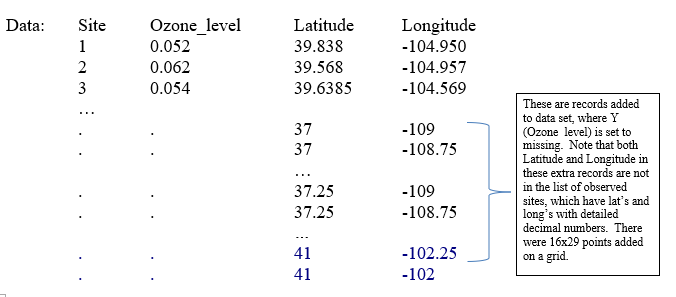
\includegraphics[width=0.7\linewidth]{figs_L22/f2} \end{center}
\end{frame}

\begin{frame}{Basic code:}
\protect\hypertarget{basic-code}{}
\begin{center}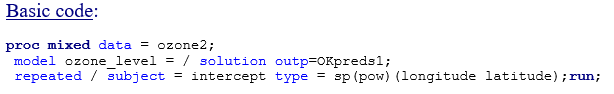
\includegraphics[width=0.7\linewidth]{figs_L22/f3} \end{center}

\begin{block}{A few notes:}
\protect\hypertarget{a-few-notes}{}
We are only fitting a fixed intercept in the model. However, predicted
values will have variability since they will all have missing Y; but
when correlations between missing and observed points or residuals are
small, predicted values will tend to default back to the fixed intercept
estimate.

The `subject=intercept' means that we have 1 ``subject'', or process.

The spatial power covariance structure is employed, using Euclidian
distances based on specific latitudes and longitudes. The observed R
matrix has nobs rows and columns, with (\(i,\ j\))th element equal to
\(\sigma_\epsilon^2 \rho^(d_{ij})\); \(d_{ij}\) is the Euclidian
distance between 2 lat/long pairs corresponding to the 2 records being
considered.

Dimensions of matrices and vectors in
\(\pmb {\hat Y}_m=\pmb X_m \pmb {\hat \beta}+\pmb {\hat R}_{mo} \pmb {\hat R}_o^{-1} (\pmb Y_o- \pmb X_o \pmb {\hat \beta})\)

In our data, there were \(16\times 29=464\) points on a grid and data
collected from 47 sites.

\(\pmb {\hat Y}_m\) and \(\pmb X_m\) are \(464\times 1\) \(\pmb Y_o\)
and \(\pmb X_o\) are \(47\times 1\) \(\pmb {\hat \beta}\) is
\(1\times 1\) \(\pmb {\hat R}_{mo}\) is \(464\times 47\)
\(\pmb {\hat R}_o^{-1}\) is \(47\times 47\)
\end{block}
\end{frame}

\begin{frame}{}
\protect\hypertarget{section-11}{}
For the spatial power structure, the (\(i,\ j\))th element of
\(\pmb {\hat R}_{mo}\) is the correlation between the new point \(i\)
and observed point \(j({\hat \rho}^{d_{ij}})\) based on distance between
the points (\(d_{ij}\)), times the estimated residual variance
(\(\hat \sigma _\epsilon^2\)).

Fits for the ozone data considering several different time points
follow.
\end{frame}

\begin{frame}{}
\protect\hypertarget{section-12}{}
\begin{center}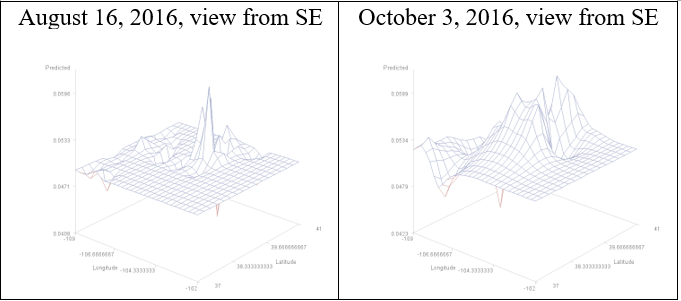
\includegraphics[width=0.7\linewidth]{figs_L22/f4} \end{center}

Higher ozone is apparent near Denver and along front range; some lower
values apparent in the west.

The estimated correlation parameter for the analysis on the left was
relatively small, resulting in sharper peaks; the one on the right was
relatively large, resulting in more gradual changes.

The view is from the southeast, as if you were flying in from Texas.
\end{frame}

\begin{frame}{}
\protect\hypertarget{section-13}{}
\begin{center}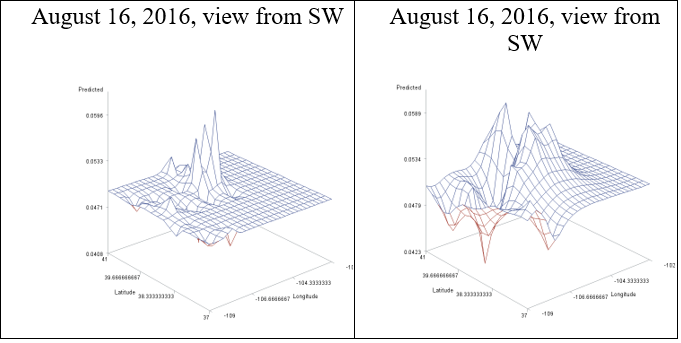
\includegraphics[width=0.7\linewidth]{figs_L22/f5} \end{center}

For a 3D plot, sometimes it helps to have a view from another angle.
This is looking from the Southwest (as if you were flying in from San
Diego). The dip on the western slope is more noticeable here.
\end{frame}

\begin{frame}{Monitoring locations}
\protect\hypertarget{monitoring-locations}{}
\begin{center}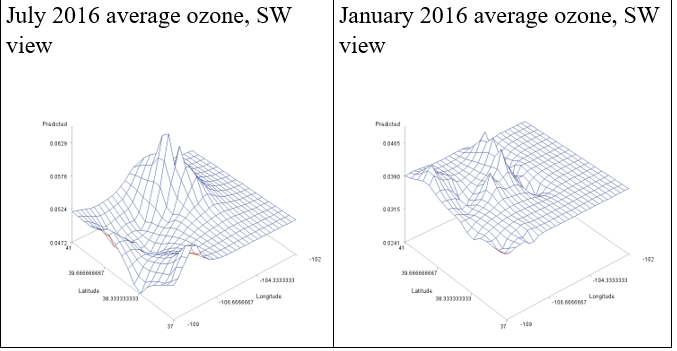
\includegraphics[width=0.7\linewidth]{figs_L22/f6} \end{center}

The figures demonstrate higher summer ozone in Denver (also note
scales).

\begin{center}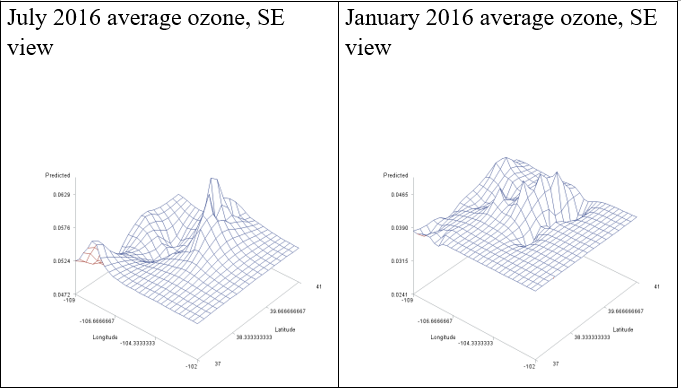
\includegraphics[width=0.7\linewidth]{figs_L22/f7} \end{center}

Same graphs, different views
\end{frame}

\begin{frame}{Estimates of parameters in models}
\protect\hypertarget{estimates-of-parameters-in-models}{}
\begin{center}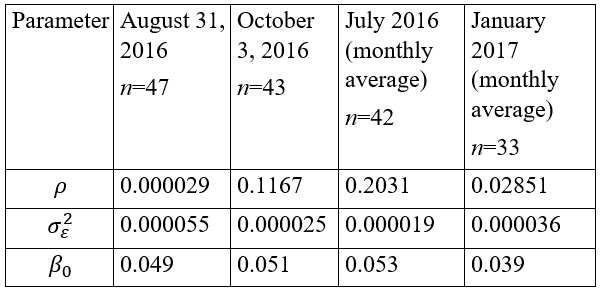
\includegraphics[width=0.7\linewidth]{figs_L22/f8} \end{center}

A slightly more advanced analysis, universal kriging, uses the same BLUP
for as previously described, but adds more predictors to the model than
just the fixed intercept.
\end{frame}

\begin{frame}{Some other article/software references for spatial
analyses:}
\protect\hypertarget{some-other-articlesoftware-references-for-spatial-analyses}{}
Guillas and Lai (2010), Bivariate splines for spatial functional
regression models. Applications also involve ozone data.

geoRglm: A Package for Generlised Linear Spatial Models. It is an R
package that employs MCMC.

PROC KRIG2ED in SAS
\end{frame}

\hypertarget{semi-variograms}{%
\section{Semi-variograms}\label{semi-variograms}}

\begin{frame}{Semi-variograms}
\protect\hypertarget{semi-variograms-1}{}
The semi-variogram is used to determine how the strength of the
relationship between responses depends on the space between the points.
It can also be used if time is the dimension of interest (i.e., for
longitudinal data rather than spatial data).

The semi-variogram is inversely related to the covariance function;
typically the covariance function will decrease as the space between
measures increases, while the semi-variogram increases.

An empirical-based version of the semi-variogram uses the data without
parametric constraints in order to understand the covariance; a
model-based version assumes some parametric structure, and estimates the
parameters using the data.
\end{frame}

\begin{frame}{Example of semi-variograms using model-based forms}
\protect\hypertarget{example-of-semi-variograms-using-model-based-forms}{}
\begin{center}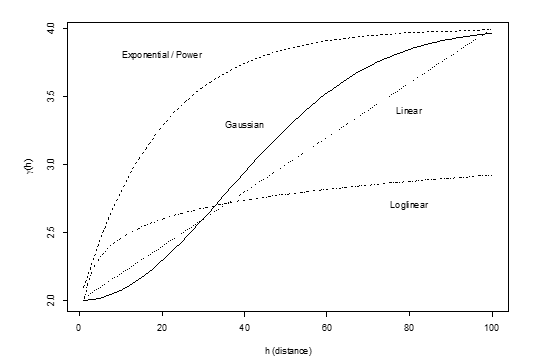
\includegraphics[width=0.7\linewidth]{figs_L22/f9} \end{center}
\end{frame}

\begin{frame}{Application:}
\protect\hypertarget{application-1}{}
Raw FEV1 for children at the NJH school (2003-04); here the
semi-variogram is constructed for time between measures.

\begin{center}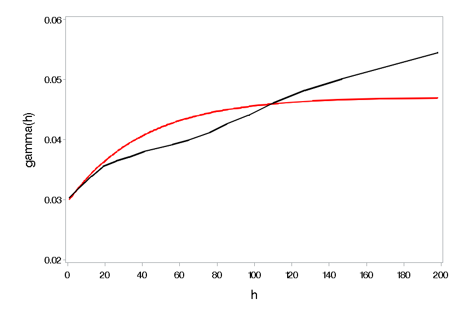
\includegraphics[width=0.7\linewidth]{figs_L22/f10} \end{center}

The empirical variogram function (black) shows a fairly linear increase
(LOESS used an AICC selected value of 0.36 for the fit). The red curve
is the fitted semi-variogram based on a PROC MIXED fit using the spatial
power function.
\end{frame}

\hypertarget{summary}{%
\section{Summary}\label{summary}}

\begin{frame}{Summary}
\protect\hypertarget{summary-1}{}
\end{frame}

\end{document}
